\documentclass[11pt, a4paper]{jsarticle}
\usepackage{geometry}
\usepackage{cite}
\usepackage{url}
\usepackage[dvipdfmx]{graphicx}
\usepackage{amsmath}

\geometry{left=25mm,right=25mm,top=25mm,bottom=30mm}

\title{
2024年度 応用プログラミング実験\\
テクニカルライティング\\
レポート}
\author{
学修番号: 22140026 \\
氏名: 谷 知拓 \footnote{東京都立大学 システムデザイン学部 情報科学科} \\
}
\begin{document}
\date{2024.4.12}
\maketitle
\section*{はじめに}
本稿は,2024年度応用プログラミング実験の第1回 テクニカルライティングで学んだことを確認するレポート課題である.各節の課題の解答を所定の位置に記入し,PDFファイルを出力せよ.その後,提出ファイル名を「APL\_第1回レポート\_学修番号\_氏名」としてkibacoの第1回課題に提出すること.

%%%%%%%%%%%%%%%%%%%%%%%%%%%%%%%%%%%%%%%%%%%%%%%%%%%%%%%%%%%%%%%%%
\section{パラグラフライティング}
一つのパラグラフで扱う話題は一つでなければならない.次の文を適切な順番に並べ替え,さらに3つのパラグラフにわけなさい.

\subsection{飲酒や喫煙で脳が老化(出典:Newton 2020年5月号)}
\begin{itemize}
    \item[(1)]また喫煙量が1日平均1箱増加するごとに,脳年齢は0.03歳高くなるという.
    \item[(2)]解析によると,1日あたりのアルコール摂取量が1グラムふえるごとに,脳年齢は0.02歳高くなるという.
    \item[(3)]脳の老化が進む要因には,遺伝的な要因に加えて,飲酒や喫煙といった要因があるといわれている.
    \item[(4)]一方,ほぼ毎日飲酒もしくは喫煙をする人は,脳年齢が高くなることがわかった.
    \item[(5)]しかし,飲酒や喫煙と脳の老化との具体的な関係は不明だった.
    \item[(6)]脳の変化にはさまざまな要因が関係しているため,脳を老化させる要因をより明確に把握するためにはさらにたくさんのデータを解析する必要がある,と博士らはのべている.
    \item[(7)]その結果,飲酒や喫煙の頻度が低いと,脳の老化におよぼす影響は小さかった.
    \item[(8)]アメリカ,南カルフォルニア大学のニン博士らは,イギリスのバイオバンク(病気などの研究のため,ヒト由来のさまざまな試料を保管している施設)に登録された45~81歳の被験者1万7308人分の脳画像データを使用して,飲酒や喫煙と脳年齢(脳の構造などから算出される脳の老化の指標)との関係について解析した.
\end{itemize}
%%%%%%%%%%%%%%%%%%%%%%%%%%%%%%%%%%%%%%%%%%%%%%%%%%%%%%%%%%%%%%%%%
\subsection*{1.1 解答}

以下の通り並び替え,3つのパラグラフに分ける.

\begin{itemize}
    \item[(3)]脳の老化が進む要因には,遺伝的な要因に加えて,飲酒や喫煙といった要因があるといわれている.
    \item[(5)]しかし,飲酒や喫煙と脳の老化との具体的な関係は不明だった.
    \item[] ---
    \item[(8)]アメリカ,南カルフォルニア大学のニン博士らは,イギリスのバイオバンク(病気などの研究のため,ヒト由来のさまざまな試料を保管している施設)に登録された45~81歳の被験者1万7308人分の脳画像データを使用して,飲酒や喫煙と脳年齢(脳の構造などから算出される脳の老化の指標)との関係について解析した.
    \item[(7)]その結果,飲酒や喫煙の頻度が低いと,脳の老化におよぼす影響は小さかった.
    \item[(4)]一方,ほぼ毎日飲酒もしくは喫煙をする人は,脳年齢が高くなることがわかった.
    \item[(2)]解析によると,1日あたりのアルコール摂取量が1グラムふえるごとに,脳年齢は0.02歳高くなるという.
    \item[(1)]また喫煙量が1日平均1箱増加するごとに,脳年齢は0.03歳高くなるという.
    \item[] ---
    \item[(6)]脳の変化にはさまざまな要因が関係しているため,脳を老化させる要因をより明確に把握するためにはさらにたくさんのデータを解析する必要がある,と博士らはのべている.
\end{itemize}

%%%%%%%%%%%%%%%%%%%%%%%%%%%%%%%%%%%%%%%%%%%%%%%%%%%%%%%%%%%%%%%%%
\subsection{深くもぐるクジラの謎(出典:Newton 2020年5月号)}
\begin{itemize}
\item[(1)]アカボウクジラの最大の天敵はシャチだ.
\item[(2)]普通クジラは,限られた潜水時間でできるだけたくさんのえさを摂取するために効率的な方法をとると考えられるため,アカボウクジラのような行動をとらないという.
\item[(3)]また,浅瀬に浮上してくるときは鳴き声を出さずに,えさをとっていた場所から1キロメートルはなれた場所に浮上したという.
\item[(4)]スペイン,ラ・ラグーナ大学のソト博士らの研究グループは,26頭のアカボウクジラにセンサーを取りつけ,鳴き声と泳ぎ方を記録し,分析した.
\item[(5)]博士らは,アカボウクジラはシャチにみつからないようにこのような採餌行動をとっているのではないか,と考えている.
\item[(6)]その結果,アカボウクジラは400メートル以上もぐってから少しずつ鳴き声を発することで周辺環境を把握し,えさをさがしはじめることがわかった.
\item[(7)]「アカボウクジラ」の中には,海の深いところでしかえさをとらず,海面にもどるときもゆっくりと時間をかけて泳ぐクジラがいる.
\item[(8)]シャチは,クジラの発する鳴き声をとらえることでクジラをみつけだすが,水深200メートルぐらいまでしかもぐれない.
\end{itemize}

%%%%%%%%%%%%%%%%%%%%%%%%%%%%%%%%%%%%%%%%%%%%%%%%%%%%%%%%%%%%%%%%%
\subsection*{1.2 解答}

以下の通り並び替え,3つのパラグラフに分ける.

\begin{itemize}
    \item[(7)]「アカボウクジラ」の中には,海の深いところでしかえさをとらず,海面にもどるときもゆっくりと時間をかけて泳ぐクジラがいる.
    \item[(2)]普通クジラは,限られた潜水時間でできるだけたくさんのえさを摂取するために効率的な方法をとると考えられるため,アカボウクジラのような行動をとらないという.
    \item[] ---
    \item[(4)]スペイン,ラ・ラグーナ大学のソト博士らの研究グループは,26頭のアカボウクジラにセンサーを取りつけ,鳴き声と泳ぎ方を記録し,分析した.
    \item[(6)]その結果,アカボウクジラは400メートル以上もぐってから少しずつ鳴き声を発することで周辺環境を把握し,えさをさがしはじめることがわかった.
    \item[(3)]また,浅瀬に浮上してくるときは鳴き声を出さずに,えさをとっていた場所から1キロメートルはなれた場所に浮上したという.
    \item[] ---
    \item[(5)]博士らは,アカボウクジラはシャチにみつからないようにこのような採餌行動をとっているのではないか,と考えている.
    \item[(1)]アカボウクジラの最大の天敵はシャチだ.
    \item[(8)]シャチは,クジラの発する鳴き声をとらえることでクジラをみつけだすが,水深200メートルぐらいまでしかもぐれない.
\end{itemize}

%%%%%%%%%%%%%%%%%%%%%%%%%%%%%%%%%%%%%%%%%%%%%%%%%%%%%%%%%%%%%%%%%
\newpage
\section{一文一義}
一つの文章には一つの事柄のみ書かなれけばならない.次の文章を「一文一義」に書き直しなさい.
\begin{itemize}
    \item[(1)] 本来,月はじめに集める部費ですが,明日は試験も終わることですし,ご連絡が遅くなってしまい申し訳ありませんが,今月の部費を集めさせていただきます.
    \item[(2)] 東京本社では営業にノルマと業績に応じた報酬を提供しているが,業績評価が営業の意欲を高めているのかどうかを考えてみたい.
    \item[(3)] さらに,1977年に木星と土星の探査機としてボイジャーが米航空宇宙局から打ち上げられた時にも,未知の宇宙文明と遭遇する場合に備えて地球からのいろいろな情報とともに,一時間半にわたって多くの音楽がLP化されて搭載されたが,その中心に選ばれたものもバッハの$<<$ブランデンブルク協奏曲第二番$>>$第一楽章であった.
\end{itemize}
%%%%%%%%%%%%%%%%%%%%%%%%%%%%%%%%%%%%%%%%%%%%%%%%%%%%%%%%%%%%%%%%%
\subsection*{2 解答}

以下の通り,それぞれの文章を「一文一義」に書き直す.

\begin{itemize}
    \item[(1)] 本来,月はじめに集める部費ですが,まだ集めていません.明日で試験が終わります.そのため,明日に今月の部費を集めさせていただきます.ご連絡が遅くなり申し訳ありません.
    \item[(2)] 東京本社では営業にノルマと業績に応じた報酬を提供している.そこで,業績評価が営業の意欲を高めているのかどうかを考えてみたい.
    \item[(3)] さらに,1977年に木星と土星の探査機としてボイジャーが米航空宇宙局から打ち上げられた.その時にも,未知の宇宙文明と遭遇する場合に備えて,地球からのいろいろな情報とともに,一時間半にわたって多くの音楽がLP化されて搭載された.そして,その中心に選ばれたものもバッハの$<<$ブランデンブルク協奏曲第二番$>>$第一楽章であった.
\end{itemize}

%%%%%%%%%%%%%%%%%%%%%%%%%%%%%%%%%%%%%%%%%%%%%%%%%%%%%%%%%%%%%%%%%
\newpage
\section{まぎれのない文}
次の文は二通りの意味に読める.二つの意味を説明しなさい.さらに各意味が一意に決まるように文を書き直しなさい.
\begin{itemize}
    \item[(1)] AさんとBさんは高校時代からの親友です.
    \item[(2)] すべての増幅器は安定でない.
    \item[(3)] 整数$-2$,$-1$,$0$,$1$のうちで絶対値最大の値を$a$とする.
    \item[(4)] 新しく造られた自立式電波塔,東京○○○ツリーは世界一の高さではない.
\end{itemize}
%%%%%%%%%%%%%%%%%%%%%%%%%%%%%%%%%%%%%%%%%%%%%%%%%%%%%%%%%%%%%%%%%
\subsection*{3 解答}

\begin{itemize}
    \item[(1)] 「AさんとBさんは,私が高校時代からの親友です.」と「AさんとBさんは,彼/彼女らが高校時代からの親友です.」の 2 通り
    \item[(2)] 「増幅器はすべて安定でない.」と「必ずしもすべての増幅器は安定でない.」
    \item[(3)] 「整数$-2$,$-1$,$0$,$1$の絶対値の値を$a$とする.」と「整数$-2$,$-1$,$0$,$1$のうちで絶対値最大の値を$a$とする.」
    \item[(4)] 「新しく造られた自立式電波塔は世界一の高さではなく,東京○○○ツリーも世界一の高さではない.」と「新しく造られた自立式電波塔である東京○○○ツリーは世界一の高さではない.」
\end{itemize}

%%%%%%%%%%%%%%%%%%%%%%%%%%%%%%%%%%%%%%%%%%%%%%%%%%%%%%%%%%%%%%%%%
\newpage
\section{複文の弊害}
複文は,意味の曖昧さや,主語と述語の不一致など,弊害が起こりやすい.単文を中心となるように,次の文を,短い文にまとめ,さらにそれらを論理的につなげなさい.
\begin{itemize}
    \item[(1)] いくら理想の道路を造ろうと,起終点は人々の居住生活圏の中にある以上,そして現実に日本の道路は基幹道路といえども居住地域のコミュニティ内を通らざるを得ない以上,自動車の走行速度は,スピードに適応能力のない人々の住む地域なるがゆえに,それが危機感を与えずにはいられない.

    \item[(2)] 携帯電話の需要が固定電話のそれを上回るようになって久しいが,かつて固定電話には,加入権についての財産的価値や,対外的な信用性があったことなどから,いまだに中高年のあいだではそれを維持しようとする意識が強いようであり,確かに,災害時における信頼性が高いなどの長所もあるから,必ずしも携帯電話が万能ではないという主張には,一定の説得力があるように思われるものの,携帯電話の著しい普及の背景には,携行性の向上だけでなくスマートフォンに代表される高機能化への支持があったことを忘れてはならないし,年配者や障害者の生活支援といった従来の固定電話にはない大きな可能性を持っているのである.
\end{itemize}
%%%%%%%%%%%%%%%%%%%%%%%%%%%%%%%%%%%%%%%%%%%%%%%%%%%%%%%%%%%%%%%%%
\subsection*{4 解答}

\begin{itemize}
    \item[(1)] 起終点は人々の居住生活圏の中にあり,そして現実に日本の道路は基幹道路といえども居住地域のコミュニティ内を通らざるを得ない.なので,自動車の走行速度は,スピードに適応能力のない人々の住む地域なる.そのため,いくら理想の道路を造ろうと,それが危機感を与えずにはいられない.

    \item[(2)] 携帯電話の需要が固定電話のそれを上回るようになって久しい.しかし,かつて固定電話には,加入権についての財産的価値や,対外的な信用性があったことなどから,いまだに中高年のあいだではそれを維持しようとする意識が強い.確かに,災害時における信頼性が高いなどの長所もあるから,必ずしも携帯電話が万能ではないという主張には,一定の説得力があるように思われる.だが,携帯電話の著しい普及の背景には,携行性の向上だけでなくスマートフォンに代表される高機能化への支持があったことを忘れてはならない.また,年配者や障害者の生活支援といった従来の固定電話にはない大きな可能性を持っているのである.
\end{itemize}

%%%%%%%%%%%%%%%%%%%%%%%%%%%%%%%%%%%%%%%%%%%%%%%%%%%%%%%%%%%%%%%%%
\newpage
\section{事実と意見}
事実を書いているのか,意見を書いているのかをいつも意識して,両者を明らかに区別して書かなければならない.
\begin{itemize}
    \item 事実とは,証拠をあげて裏付けすることができるものである.すなわち,自然に起こる事象や自然法則,過去に起こった,人間の関与した事件などの記述で,然るべきテストや調査によって真偽を客観的に確認できるものである.事実は真実とは限らない.
    \item 意見は広い概念で,推論,判断,狭義の意見,確信,仮説,理論(法則は事実)を含む.
\end{itemize}
以上のことを踏まえて,次の問に答えなさい.

\subsection{事実の記述}
事実の記述として不適切なものを選び,なぜ不適切なのかを説明しなさい.次にそれらの文について,事実を記述する文に書き直しなさい.
\begin{itemize}
    \item[(1)] クイックソートは最も優れたアルゴリズムのひとつである.
    \item[(2)] その実験で得られた数値から,おぼろげながら問題の物質が何であるか特定された.
    \item[(3)] 最も広く普及したマイコンとして歴史に名を残したプロセッサ"pettanko"の命令セットアーキテクチャは,インテローラ社のXZ-680のそれを拡張したものと考えることができる.
\end{itemize}
%%%%%%%%%%%%%%%%%%%%%%%%%%%%%%%%%%%%%%%%%%%%%%%%%%%%%%%%%%%%%%%%%
\subsection*{5.1 解答}

\begin{itemize}
    \item[(3)] 最も広く普及したマイコンとして歴史に名を残したプロセッサ"pettanko"の命令セットアーキテクチャは,インテローラ社のXZ-680のそれを拡張したものと考えることができる.
\end{itemize}

理由 : 事実ではなく,意見となっている.検証可能な事柄であれば,事実確認をし,事実として記載するべきである.

最も広く普及したマイコンとして歴史に名を残したプロセッサ"pettanko"の命令セットアーキテクチャは,インテローラ社のXZ-680のそれを拡張したものである.

%%%%%%%%%%%%%%%%%%%%%%%%%%%%%%%%%%%%%%%%%%%%%%%%%%%%%%%%%%%%%%%%%

\subsection{意見の記述}
意見の記述として不適切なものを選びなさい.
\begin{itemize}
\item[(1)] 私は,これが最良の方法だと思う.
\item[(2)] これが最良の方法である.
\item[(3)] この色はあの色より赤っぽい.
\item[(4)] 故障の原因は接続ミスであった.
\end{itemize}
%%%%%%%%%%%%%%%%%%%%%%%%%%%%%%%%%%%%%%%%%%%%%%%%%%%%%%%%%%%%%%%%%
\subsection*{5.2 解答}

(1), (4)


%%%%%%%%%%%%%%%%%%%%%%%%%%%%%%%%%%%%%%%%%%%%%%%%%%%%%%%%%%%%%%%%%
\newpage
\subsection{グラフから読み取れる事実}
図\ref{fig:arai}に,日本におけるインターネット利用者数および人口普及率の推移を示す.下記の例文について,グラフから読み取れる事実の記述として適切かどうかを判断しなさい.
\begin{itemize}
\item[(1)] インターネット利用者数は,2012年から2013年にかけて大幅に増加した.
\item[(2)] 2016年の人口普及率は,2006年の人口普及率に対して10.9$\%$増加し,83.5$\%$となった.
\item[(3)] 2017年には,インターネット利用者数は1億2千万人を突破し,人口普及率は85$\%$を超える.
\item[(4)] インターネット利用者数は年々増加しており,2013年に1億人を超えた.
\end{itemize}
\hspace{1em}

\begin{figure}[h]
\vspace{-5mm}
\centering
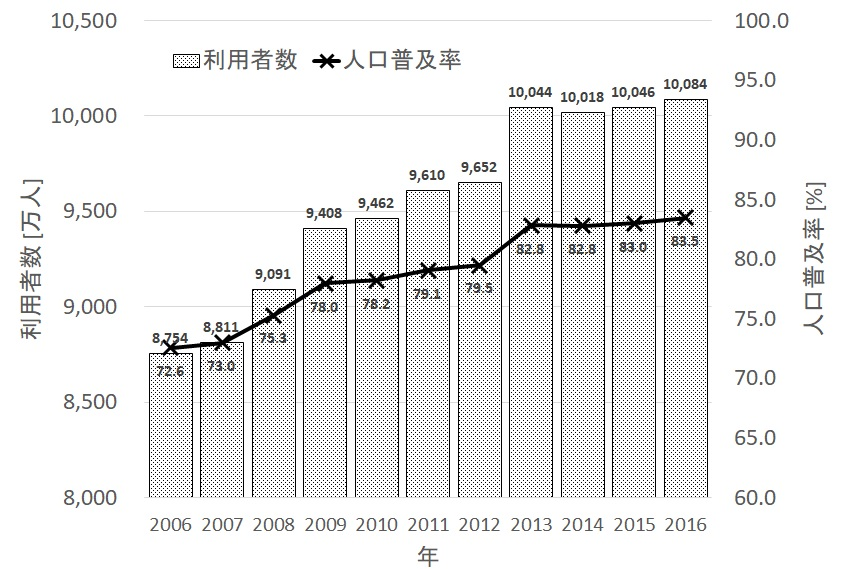
\includegraphics[width=0.9\linewidth]{internet.jpg}
\caption{日本におけるインターネット利用者数および人口普及率の推移}(出典:総務省 通信利用動向調査 平成29年調査)
\label{fig:arai}
\end{figure}
%%%%%%%%%%%%%%%%%%%%%%%%%%%%%%%%%%%%%%%%%%%%%%%%%%%%%%%%%%%%%%%%%
\subsection*{5.3 解答}

以下に,回答する.

\begin{itemize}
    \item[(1)] 適切
    \item[(2)] 適切
    \item[(3)] 不適切
    \item[(4)] 不適切
\end{itemize}

%%%%%%%%%%%%%%%%%%%%%%%%%%%%%%%%%%%%%%%%%%%%%%%%%%%%%%%%%%%%%%%%%
\newpage
\section{数式入力の練習}
図\ref{fig:eqs}に示した数式を\LaTeX または,MS Wordの数式モードで記載せよ.数式モードの使い方は各自で調べること.

\begin{figure}[h]
\centering
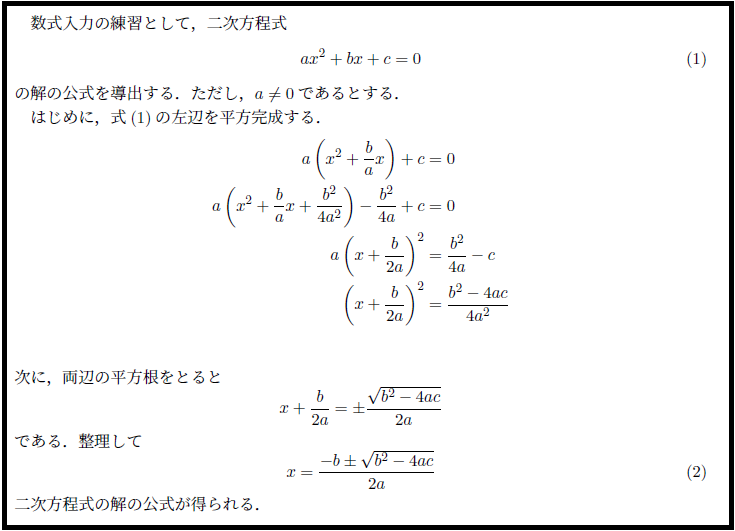
\includegraphics[width=0.9\linewidth]{eqs.png}
\caption{数式入力の練習}
\label{fig:eqs}
\end{figure}

%%%%%%%%%%%%%%%%%%%%%%%%%%%%%%%%%%%%%%%%%%%%%%%%%%%%%%%%%%%%%%%%%
\subsection*{6 解答}

以下に,数式を\LaTeX で記載する.

\rule{\linewidth}{0.1mm}

数式入力の練習として,二次方程式

\begin{equation}
    ax^2 + bx + c = 0
    \label{eq:eq1}
\end{equation}

の解の公式を導出する.ただし, $a \neq 0$ であるとする.

はじめに,式 \ref{eq:eq1} の左辺を平方完成する.

\begin{equation}
    \begin{aligned}
    a\left(x^2+\frac{b}{a} x\right)+c & =0 \\
    a\left(x^2+\frac{b}{a} x+\frac{b^2}{4 a^2}\right)-\frac{b^2}{4 a}+c & =0 \\
    a\left(x+\frac{b}{2 a}\right)^2 & =\frac{b^2}{4 a}-c \\
    \left(x+\frac{b}{2 a}\right)^2 & =\frac{b^2-4 a c}{4 a^2}
    \end{aligned}
\end{equation}

次に,両辺の平方根をとると

\begin{equation}
    x+\frac{b}{2 a}= \pm \frac{\sqrt{b^2-4 a c}}{2 a}
\end{equation}

である.整理して

\begin{equation}
    x=\frac{-b \pm \sqrt{b^2-4 a c}}{2 a}
\end{equation}

二次方程式の解の公式が得られる.

\rule{\linewidth}{0.1mm}

%%%%%%%%%%%%%%%%%%%%%%%%%%%%%%%%%%%%%%%%%%%%%%%%%%%%%%%%%%%%%%%%%
\section*{おわりに}

「事実は真実とは限らない」という点が印象的であった.科学的根拠や客観的に確認できる証拠があると,私たちは,それらから合理的に導かれる理論を,「真実である」と捉えて疑わないきらいがあるが,実際にはそれが必ずしも「真実」とは限らない.
過去にも,当時は「科学的」「合理的」と謳われた理論が,後の世に,誤っていたことが指摘されることはいくども繰り返されてきた.これは,今日に至るまで人類が,理論や科学技術をつねに発展させてきた賜物であるが,その一方で今の時点で,もっとも合理的に導かれた理論が,あくまで今見える世界に基づいた,『暫定的な"真実"』であることを忘れてはならないと感じた.


% 参考文献を以下に記載する
\bibliographystyle{junsrt} 
\begin{thebibliography}{99}
    \bibitem{okumura} 奥村晴彦,黒木裕介『\LaTeX 美文書作成入門』第9版(技術評論社,2023)
    \bibitem{abcde} このように,参考文献を必要に応じて追記すること.
\end{thebibliography}

\end{document}